\newcommand*\circled[2][black]{\tikz[baseline=(char.base)]{
    \node[scale=0.85pt,shape=circle, thin,draw=#1!60, fill=#1!5,inner sep=0.1pt] (char) {#2};}}

\tikzset{
    dot diameter/.store in=\dot@diameter,
    dot diameter=2pt,
    dot spacing/.store in=\dot@spacing,
    dot spacing=16pt,
    dots/.style={
        line width=\dot@diameter,
        line cap=round,
        dash pattern=on 0pt off \dot@spacing,
    }
}


\section{Neural Mass Models}\label{sec:neural-mass-models}
\todo{slightly deeper introduction (we already have this in the EEG section) to NMMs in general}

\subsection{The Jansen-Rit Model}\label{subsec:the-jansen-rit-model}

The widely used Jansen-Rit Model~\cite{jansen_neurophysiologically-based_1993, jansen_electroencephalogram_1995},
is based on earlier models by Wilson \& Cowan~\cite{wilson_excitatory_1972},
Lopes da Silva et al.~\cite{lopes_da_silva_model_1974, lopes_da_silva_models_1976} and
Zetterberg et al.~\cite{zetterberg_performance_1978}.
It represents a cortical column in the brain, which is made up of three main components,
each modeling a population of neurons with distinct characteristics.

The basic schema of the model is visualized in Fig.~\ref{fig:Jansen Rit Flowchart}, showing the connections
\begin{wrapfigure}{r}{0.5\textwidth}
    \begin{tikzpicture}[
		roundein/.style={circle, draw=green!60, fill=green!5, very thick, minimum size=11mm},
		roundiin/.style={circle, draw=red!60, fill=red!5, very thick, minimum size=11mm},
		rectp/.style={rectangle, rounded corners=2mm, draw=green!60, fill=green!5, very thick},
		trinode/.style={isosceles triangle, isosceles triangle apex angle=60, very thick, draw=cyan!60, shape border rotate=270, fill=cyan!5,},
		]
        
        \pgfdeclarelayer{bg}
        \pgfsetlayers{bg,main}
        
		%Nodes
		
		\node[trinode]    (PC)        {PC};
		\node[roundein]   (EIN)  [above left= 0.5cm and 2.25cm of PC.center] {EIN};
		\node[roundiin]   (IIN) [above right= 0.5cm and 2.25cm of PC.center] {IIN};
		\node[rectp]   (p) [above left=3cm and 1cm of PC.north] {Ext.};
		\node[below= 0.5cm of PC] (pc_out){};
		\node[above= 0.2cm of EIN.north] (ein_out){};
		\node[above= 0.2cm of IIN.north] (iin_out){};
		%Lines
		\draw[-, red] (IIN.north) -- (iin_out.center){};
		\draw[-, green] (EIN.north) -- (ein_out.center){};
		
		\draw[-{Stealth[scale=1.5]}, red] (iin_out.center) -| (PC.30) node[near end, right, black](output){$\circled[red]{$-$}$};
		\draw[-{Stealth[scale=1.5]}, green] (ein_out.center) -| (PC.155) node[near end, left, black](output){$\circled[green]{$+$}$};
		\draw[-{Stealth[scale=1.5]}, green] (p.east) -| (PC.140) node[pos=0.888, right, black](output){$\circled[green]{$+$}$};
		
		
		\draw[-, green] (PC.south) -- (pc_out.center){};% node[near start, right](output){$\circled{$+$}$};
		
		\draw[-{Stealth[scale=1.5]}, green] (pc_out.center) -| (EIN.south){} node[pos=0.85, right, black](output){$\circled[green]{$+$}$};
		\draw[-{Stealth[scale=1.5]}, green] (pc_out.center) -| (IIN.south){} node[pos=0.85, left, black](output){$\circled[green]{$+$}$};
        
        \begin{pgfonlayer}{bg}
        
        
        \filldraw [fill=darkgray!5,draw=darkgray]
            ($ (EIN.west) + (-0.2,1.7) $)
            rectangle ($ (IIN.east) + (0.2,-3) $);
        \node [above left=1.35cm and 0.2 of EIN.west, anchor=west, text=darkgray]{Cortical Column};
        \end{pgfonlayer}
		
	\end{tikzpicture}
    \caption{\textbf{Basic Schema of the Jansen-Rit Model:} Three populations of neurons}
    \label{fig:Jansen Rit Flowchart}
\end{wrapfigure}
between the main components.
There is a population of Pyramidal Cells which receives input from two populations of inter-neurons,
one of which is excitatory while the other is inhibitory.
Each of the inter-neuron-populations receives the output of the PC population.
Additionally, there is external excitatory input to the PC population from other regions of the brain.

The Block Diagram (Fig. \ref{fig:Jansen Rit Simple}) shows the individual modules of the model.
A population consists of two types of blocks:
The \textit{PSP-Block} models the behavior of the synapses and neuronal somata.
It can be either excitatory or inhibitory and converts the incoming average pre-synaptic pulse density to
an average post-synaptic membrane potential by convolving it with an
impulse response function ($h_e(t)$ and $h_i(t)$, for excitation and inhibition respectively).
The second block (sometimes called \textit{Potential-To-Rate-Block} after it's functionality)
calculates the populations response to this stimulation, transforming the incoming
average membrane potential back into an average pulse density of action potentials.
It may be roughly viewed as a functional counterpart to the axon hillock by establishing a firing threshold
and is usually implemented by a Sigmoid Function ($Sigm$).
External input from other regions of the brain is represented by $p(t)$.
The Connectivity Constants $C_1$, $C_2$, $C_3$ and $C_4$ are a proportional representation of the
average number of synapses between the populations.
The signal most closely related to the EEG and therefore the variable of interest,
is the summed average membrane potential of the PC population ($y_1(t)-y_2(t)$ in Fig.~\ref{fig:Jansen Rit Simple}).

\todo{explain neurophysiology why $EEG \approx y_1-y_2$, or reference back to explanation in EEG section}\\[1em]

\begin{figure}[H]
    \centering
    \begin{tikzpicture}[
        pc/.style={draw=black!80},
        ein/.style={draw=black!80},
        iin/.style={draw=black!80},
        pcLabel/.style={font=\small,text=black},
        einLabel/.style={font=\small,text=black},
        iinLabel/.style={font=\small,text=black},
        rectNode/.style={draw=black!80, thick},
        roundNode/.style={circle, draw=black!80, thick},
        ]
	    
 % Nodes
\node[rectNode, pc] (SigmPC) [label={[pcLabel]:PC}] {$Sigm$};
\node[rectNode, pc] (PSPPC) [right=1.8cm of SigmPC.east]{$h_e(t)$};
\node[rectNode, ein] (SigmEIN) [above=2cm of SigmPC.center, label={[einLabel]:EIN}]{$Sigm$};
\node[rectNode, iin] (SigmIIN) [below=2cm of SigmPC.center, label={[iinLabel]:IIN}]{$Sigm$};
\node[rectNode, ein] (PSPEIN) [above left= 0.5cm and 2cm of SigmPC.west]{$h_e(t)$};
\node[rectNode, iin] (PSPIIN) [below left= 0.5cm and 2cm of SigmPC.west]{$h_i(t)$};
\node[rectNode, rounded corners=3mm, ein] (ext) [left=2cm of PSPEIN.west, label={[einLabel]:Ext.}]{$p(t)$};
\node (inpIPSP) [left=0.8cm of PSPIIN.west]{};
\node (outPPSP) [right=1.2cm of PSPPC.east]{};
\node[roundNode, ein] (c1) [right=2cm of SigmEIN.east]{$C_1$};
\node[roundNode, ein] (c2) [left=2cm of SigmEIN.west]{$C_2$};
\node[roundNode, iin] (c3) [right=2cm of SigmIIN.east]{$C_3$};
\node[roundNode, iin] (c4) [left=2cm of SigmIIN.west]{$C_4$};

% add PC
\node[roundNode, pc] (addPC) [left=0.8cm of SigmPC.west]{};
\draw[-, black!80, thick, pc] (addPC.north west) -- (addPC.south east);
\draw[-, black!80, thick, pc] (addPC.north east) -- (addPC.south west);
% add Excitatory
\node[roundNode, ein] (addExc) [left=0.8cm of PSPEIN.west]{};
\draw[-, black!80, thick, ein] (addExc.north west) -- (addExc.south east);
\draw[-, black!80, thick, ein] (addExc.north east) -- (addExc.south west);

% add PC -> Sigm PC -> PSP PC
\draw[-{Stealth[scale=1.5]}, pc] (addPC.east) -- (SigmPC.west)node[coordinate, pos=0.3](measurepoint){};
\draw[-{Stealth[scale=1.5]}, pc] (SigmPC.east) -- (PSPPC.west);

% PSP PC -> y0
\draw[-{Stealth[scale=1.5]}, pc] (PSPPC.east) -- (outPPSP.center) node[pos=0.5, above, pcLabel]{\small$y_0(t)$};

% y0 -> C1 -> Sigm EIN
\draw[-{Stealth[scale=1.5]}, ein, fill=none] (outPPSP.center) |- (c1.east);
\draw[-{Stealth[scale=1.5]}, ein] (c1.west) -- (SigmEIN.east);

% y0 -> C3 -> Sigm IIN
\draw[-{Stealth[scale=1.5]}, iin, fill=none] (outPPSP.center) |- (c3.east);
\draw[-{Stealth[scale=1.5]}, iin] (c3.west) -- (SigmIIN.east);


% Sigm EIN -> c2 -> add EXC
\draw[-{Stealth[scale=1.5]}, ein] (SigmEIN.west) -- (c2.east);
\draw[-{Stealth[scale=1.5]}, ein, fill=none] (c2.west) -| (addExc.north) node[pos=0.9, right]{\small$+$};
% external -> add EXC
\draw[-{Stealth[scale=1.5]}, ein] (ext.east) -- (addExc.west) node[pos=0.9, above]{\small$+$};

% add EXC -> PSP EIN
\draw[-{Stealth[scale=1.5]}, ein] (addExc.east) -- (PSPEIN.west);
% PSP EIN -> add PC
\draw[-{Stealth[scale=1.5]}, ein, fill=none] (PSPEIN.east) -| (addPC.north) node[pos=1, left]{\small$+$} node[pos=0.4, above, einLabel]{\small$y_1(t)$};

% Sigm IIN -> C4 -> PSP IIN
\draw[-{Stealth[scale=1.5]}, iin] (SigmIIN.west) -- (c4.east);
\draw[-, iin, fill=none] (c4.west) -| (inpIPSP.center);
\draw[-{Stealth[scale=1.5]}, iin] (inpIPSP.center) -- (PSPIIN.west);
% PSP IIN -> add PC
\draw[-{Stealth[scale=1.5]}, iin, fill=none] (PSPIIN.east) -| (addPC.south) node[pos=1, left]{\small$-$} node[pos=0.4, below, iinLabel]{\small$y_2(t)$};

% electrode
\draw (measurepoint.north) -- (-1.1,1)node[coordinate,pos=0.9](a){} -- (-0.8,0.9)node[coordinate, pos=0.5](b){} -- cycle;
\node (signal)[above right=0.2cm and 2.1cm of a]{\tiny recorded Signal};
\draw (b.center) |- (signal.west);



\end{tikzpicture}
    \caption{\textbf{Simple Block Diagram after \parencite{jansen_electroencephalogram_1995}:} It's structure might be somewhat confusing when trying to visualize the biological analogy, where each population would have individual afferent PSP-Blocks. However, the fact that the two interneuron populations share a single excitatory PSP Block, because it produces identical results for both of them (disregarding their individual connectivity factor, which is simply applied afterwards), is a computational performance gain, thus likely explaining the authors' choice.}
    \label{fig:Jansen Rit Simple}
\end{figure}

\subsubsection{Potential-To-Rate Block}
For a neuron to fire an action potential, its membrane potential needs to surpass a certain threshold.
Since we are modeling not a single neuron but a whole population, we need an operator that can transform
the mean membrane potential that the neurons of the population receive as input into an average firing rate
for the whole population.
While neurons within the population may have individual firing-threshold%TODO:[citation-needed],
it can be assumed due to their sheer number, that these thresholds are normally distributed around some mean value $v_0$. %TODO:[citation-needed]
An additional assumption that this approach rests on, is that the number of afferent (i.e. incoming) connections to the individual neurons is sufficiently large to justify the assertion that all neurons receive roughly the same stimulation.
This must be modeled by a monotonically increasing function.
The Potential-To-Rate Block represents this process with a Sigmoid.
After multiple iterations by Zetterberg \cite{zetterberg_performance_1978}, Lopes da Silva \cite{lopes_da_silva_models_1976} and others, Jansen and Rit \cite{jansen_neurophysiologically-based_1993, jansen_electroencephalogram_1995} landed on the following equation:
\begin{align}
    Sigm(v) = \frac{2e_0}{1+e^{r(v_0-v)}} \label{eq:SigmJansenRit}
\end{align}
The parameter values (Table \ref{table:sigmoid_params}) are empirically determined \parencite{jansen_neurophysiologically-based_1993}. The maximum firing rate the population can achieve is set at $5 Hz$. A mean membrane potential of $6 mV$ (equal to the populations average firing threshold) elicits half of the maximum firing rate, while $\frac{0.56}{mV}$ defines the steepness. The plot in Fig. \ref{fig:Sigmoid} visualizes these properties.
%TODO: mention refractory period
\begin{table}[H]
    \centering
    \begin{tabular}{ |c|c|c|c| }
        \hline
        \multicolumn{2}{|c|}{Parameter} & Default Value & Unit \\
        \hline
        \hline
        half of maximum firing rate & \(e_0\) & \(2.5\)  & \(Hz\)      \\
        \hline
        average firing threshold    & \(v_0\) & \(6.0\)  & \(mV\)      \\
        \hline
        sigmoidal steepness         & \(r\)   & \(0.56\) & \(mV^{-1}\) \\
        \hline
    \end{tabular}
    \caption{Parameters of the Sigmoid Function}
    \label{table:sigmoid_params}
\end{table}

\begin{figure}[H]

    \centering
    \pgfplotsset{compat = newest}
    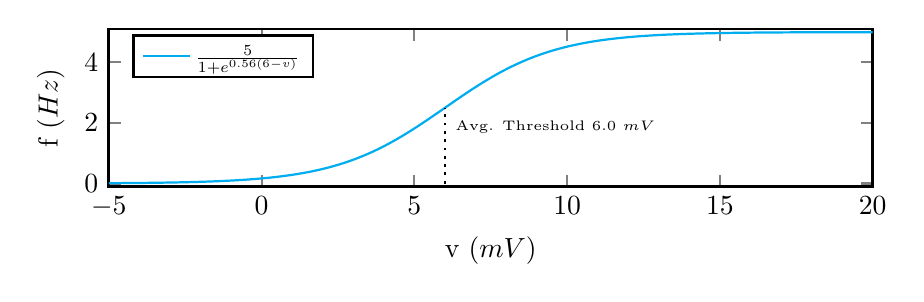
\begin{tikzpicture}
        \begin{axis}
            [
            xmin = -5, xmax = 20,
            ymin = -0.1, ymax = 5.1,
            xlabel = {v ($mV$)},
            ylabel = {f ($Hz$)},
            legend pos=north west,
            legend style={nodes={scale=0.8, transform shape}},
            ],
            \addplot[
                domain = -5:20,
                samples = 200,
                smooth,
                thick,
                cyan,
            ] {5/(1+exp(0.56*(6-x)))};
            \legend{\( \frac{5}{1+e^{0.56(6-v)}} \)};
            \draw [dotted] ([xshift=0.0cm]axis cs:6,0) -- ([yshift=0.0cm]axis cs:6,2.5) node[near end,right,font=\tiny]{Avg. Threshold 6.0 $mV$};
        \end{axis}
    \end{tikzpicture}

    \caption{Sigmoid (Eq. \ref{eq:SigmJansenRit}) \parencite{jansen_neurophysiologically-based_1993}} \
    \label{fig:Sigmoid}
\end{figure}

\subsubsection{PSP-Blocks}
%TODO: mention usages of LTI's in Physics, explain this better in general
In Physics, Linear Time-Invariant Systems (LTI systems) are oftentimes used to describe the response of electrical circuits to arbitrary input signals. They consist of a kernel function (or impulse-response function), that models the system's response to a single unit-impulse.
The PSP-Blocks are an LTI system, fully represented by an impulse response function. It describes a PSP relative to the onset of a pulse. Since the PSP differs depending on the type of cell (excitatory or inhibitory) there are two different impulse-response functions. The parameters for the EPSP (Eq. \ref{eq:ExcImpResJansenRit}) and IPSP (Eq. \ref{eq:InhImpResJansenRit}) are given in Table \ref{tab:psp_params}. The respective plots are visualized in Fig. \ref{fig:PSPPlot}.
%TODO: explain how the parameters can be tuned to achieve differnt results, and how that relatates to actual neurobiology
\begin{table}[H]
    \centering
    \begin{tabular}{ |c|c|c|c| }
        \hline
        \multicolumn{2}{|c|}{Parameter} & Default Value & Unit \\
        \hline
        \hline
        Exc\. max\. amplitude / $e$          & \(A\) & \(3.25\) & \(mV\) \\
        \hline
        %TODO: EXPLAIN 'LUMPED'!!!!
        Lumped repr\. of sum of exc\. delays & \(a\) & \(100\)  & \(Hz\) \\
        \hline
        Inh. max. amplitude / $e$          & \(B\) & \(22\)   & \(mV\) \\
        \hline
        Lumped repr\. of sum of inh\. delays & \(b\) & \(50\)   & \(Hz\) \\
        \hline
    \end{tabular}
    \caption{Parameters of the PSP Blocks}
    \label{tab:psp_params}
\end{table}

Excitatory impulse response:
\begin{equation}
    h_e(t) = \begin{cases}
                 Aate^{-at} & \mbox{ } t \geq 0 \\
                 0 & \mbox{ } t < 0
    \end{cases} \label{eq:ExcImpResJansenRit}
\end{equation}

Inhibitory impulse response:
\begin{equation}
    h_i(t) = \begin{cases}
                 Bbte^{-bt} & \mbox{ } t \geq 0 \\
                 0 & \mbox{ } t < 0
    \end{cases} \label{eq:InhImpResJansenRit}
\end{equation}



\begin{figure}[H]
    \centering
    \pgfplotsset{compat = newest}
    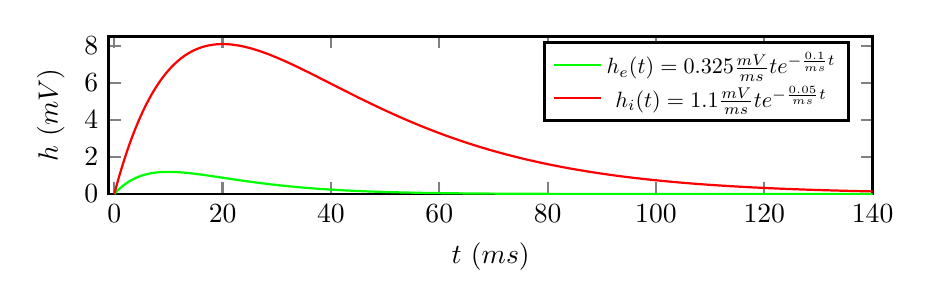
\begin{tikzpicture}
        \begin{axis}
            [
            xmin = -1, xmax = 140,
            ymin = 0, ymax = 8.5,
            xlabel = {$t$ ($ms$)},
            ylabel = {$h$ ($mV$)},
            legend pos=north east,
            legend style={nodes={scale=0.8, transform shape}},
            ],
            \addplot[
                domain = 0:140,
                samples = 200,
                smooth,
                thick,
                green,
            ] {3.25*0.1*x*e^(-0.1*x)};
            \addplot[
                domain = 0:140,
                samples = 200,
                smooth,
                thick,
                red,
            ] {22*0.05*x*e^(-0.05*x)};

            \legend{
                $h_e(t)=0.325\frac{mV}{ms} te^{-\frac{0.1}{ms}t} $,
                $ h_i(t)=1.1\frac{mV}{ms} te^{-\frac{0.05}{ms}t} $
            };

        \end{axis}
    \end{tikzpicture}

    \caption{\textbf{Impulse Response Functions:} Note the small \textcolor{green}{EPSP}  (Eq. \ref{eq:ExcImpResJansenRit}) and the large \textcolor{red}{IPSP}  (Eq. \ref{eq:InhImpResJansenRit}) \parencite{jansen_neurophysiologically-based_1993}} \
    \label{fig:PSPPlot}
\end{figure}

Jansen and Rit \cite{jansen_neurophysiologically-based_1993} justify the difference in amplitude by referencing Lopes da Silva et al. \cite{lopes_da_silva_models_1976} and stating that inhibitory neurons synapse closer to the somata of pyramidal cells (often on the cell body) than excitatory cells, increasing the effect of an inhibitory neuron about 10-fold.

\todo{maybe go more into detail about the reasons for stronger inhibition}\\[2em]
The output of the Linear System defined by the PSP-Blocks is calculated by a convolution (denoted by $\ast$) of the incoming impulse density $x(t)$ with the impulse response function $h(t)$ (Eq. \ref{eq:convolution}).
%%%%
% REMARK: CONVOLUTION
%%%%
% \begin{figure}
\begin{wrapfigure}[19]{r}{0.5\textwidth}
    \centering
    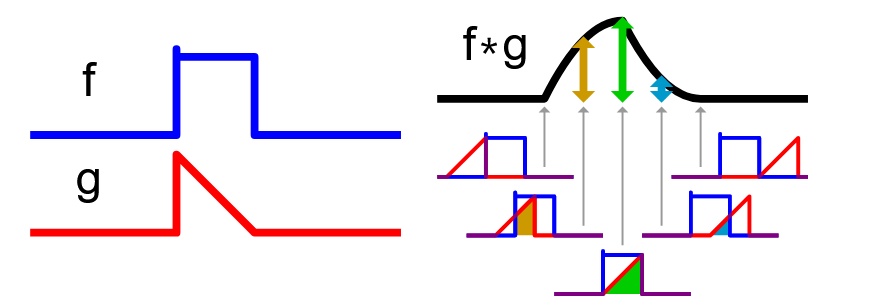
\includegraphics[width=0.30\textwidth]{Figures/convolution/wikipedia-citation-needed}
    \caption{\textbf{Convolution:} The area enclosed by $f(\tau)$ and $g(t-\tau)$ is the value of $(f\ast g)(t)$.\\
    \hrulefill \\
    \textit{By Cmglee - Own work, CC BY-SA 3.0  \url{https://commons.wikimedia.org/w/index.php?curid=20206883}}}
    % TODO: RECREATE THIS VISUALIZATION MYSELF
    \label{fig:Convolution}
\end{wrapfigure}
% \end{figure}

%\begin{minipage}{0.6\textwidth}
\begin{remark}[Convolution]
    The convolution of two functions $f(t)$ and $g(t)$ is defined as the integral of their product after one function has been reversed and shifted \footnote{There is a very intuitive explanation of convolutions by Kalid Azad on his website \url{https://betterexplained.com/articles/intuitive-convolution/}}:
    \[f(t) \ast g(t)= \int_{-\infty}^{+\infty}f(\tau)g(t-\tau) d\tau\]
    % \begin{figure}[H]
    %	\centering
    %		\pgfplotsset{,compat = newest}
    %		\begin{tikzpicture}
    %			\begin{axis}[name=plotf, height=5cm, width=5cm, ticks=none,
    %				xmin = -1, xmax = 120,
    %				ymin = 0, ymax = 9.1,
    %				legend style={nodes={scale=0.5, transform shape}},
    %				legend pos=north east,
    %				],
    %				\addplot[
    %				domain = 0:120,
    %				samples = 200,
    %				smooth,
    %				thick,
    %				green,
    %				] {1.1*x*e^(-0.05*x)};
    %				\legend{$f(\tau)$};
    %			\end{axis}
    %			\begin{axis}[name=plotg, at={($(plotf.east)+(1cm,0)$)}, anchor=west, height=5cm, width=5cm, ticks=none,
    %				legend style={nodes={scale=0.5, transform shape}},
    %				xmin = -120, xmax = 0,
    %				ymin = 0, ymax = 9.1,
    %				legend pos=north east,
    %				],
    %				\addplot[
    %				domain = -120:0,
    %				samples = 200,
    %				smooth,
    %				thick,
    %				red,
    %				] {1.1*(-x)*e^(-0.05*(-x))};
    %				\legend{$g(-\tau)$};
    %			\end{axis}
    %
    %			\begin{axis}[name=plotconv1, at={($(plotf.south)-(0,1cm)$)}, anchor=north, height=4cm, width=4cm, ticks=none,
    %				xmin = -120, xmax = 120,
    %				ymin = 0, ymax = 9.1,
    %				%legend pos=north east,
    %				],
    %				\addplot[name path=G,
    %				domain = 0:120,
    %				samples = 100,
    %				smooth,
    %				thick,
    %				green,
    %				] {1.1*x*e^(-0.05*x)};
    %				%\legend{$g(\tau)$};
    %				\addplot[name path=F,
    %				domain = -100:20,
    %				samples = 100,
    %				smooth,
    %				thick,
    %				red,
    %				] {1.1*(-x+20)*e^(-0.05*(-x+20))};
    %				%\legend{$f(\tau)$};
    %				\fill [cyan!20,
    %				intersection segments={
    %					of=F and G,
    %					sequence={R1--L2}
    %				}];
    %
    %			\end{axis}
    %		\end{tikzpicture}
    %
    %		\caption{Convolution} \
    %		\label{Fig: convolution}
    %
    %
    % \end{figure}
    If $f(t)$ is a unit-impulse $\delta(t)$ (in our case that would mean each cell of the previous population firing a single action potential at the same time) the result is just $g(t)$ (in our case representing a single full-amplitude impulse response as the mean membrane potential):
    \[\delta(t) \ast g(t)= \int_{-\infty}^{+\infty}\delta(\tau)g(t-\tau) d\tau = g(t)\]
    In the general case, this process can be used to mathematically model the integration of incoming action potential densities in the soma.\\[1em]
    Importantly, the Convolution Theorem states that the convolution of $f(t)$ and $g(t)$ becomes a simple multiplication when applying the Laplace Transform:
    \[\mathscr{L}\{f(t) \ast g(t)\}= \mathscr{L}\{f(t)\}\mathscr{L}\{g(t)\} = F(s)G(s)\]
    That means you can calculate a convolution with the inverse Laplace-Transform of the multiplication of the functions' individual Laplace-Transforms:
    \[f(t) \ast g(t)= \mathscr{L}^{-1}\{F(s)G(s)\}\]

\end{remark}
% TODO:: USE AND REFERENCE Kalid Azad's Explanation from https://betterexplained.com/articles/intuitive-convolution/
%%%%%%
%\end{minipage}
%\begin{minipage}{0.4\textwidth}

%\end{minipage} \\[1em]
Since the convolution in the time-domain is a computationally heavy operation, it is oftentimes faster to transform the equation into the Laplace-Domain (see Eq. \ref{eq:laplace_domain}), apply the Convolution Theorem and perform the multiplication there, and transform the results back to the time-domain. This results in a second order differential equation (Eq. \ref{eq:sec_ord_nmm}) that can be efficiently solved by numerical integration. To obtain this form, we need the Laplace transform $H_e(s)$ (in this context also called \textit{Transfer Function}) of our response function $h_e(t)$:
\[H_e(s) =\mathscr{L}\{h_e(t)\}  = \mathscr{L}\{Aate^{-at} \} = \frac{Aa}{(s+a)^2} = \frac{Aa}{s^2+2as+a^2}\label{eq:laplace_h_e}\]
% \begin{figure}[H]
%	\centering
%	\pgfplotsset{compat = newest}
%	\begin{tikzpicture}
%		\begin{axis}[
%			xmin = -0.07, xmax = 0.05,
%			ymin = -0.1, ymax = 100.0,
%			xlabel = {$t$ ($ms$)},
%			ylabel = {$h$ ($mV$)},
%			legend pos=north east,
%			],
%			\addplot[
%			domain = -0.07:0.05,
%			samples = 200,
%			smooth,
%			thick,
%			red,
%			] {3.25*0.01/((x+0.01)^2)};
%
%			\legend{$H_e(s) = \frac{0.325}{(s+0.01)^2}  $};
%
%		\end{axis}
%	\end{tikzpicture}
%
%	\caption{$H_e(s)$} \
%	\label{Fig: Transfer Function }
% \end{figure}
With that, we can start to transform our initial equation into the desired Second Order System:
\begin{alignat}{5}
    &                                           & &&          \overbrace{y(t)}^{\text{PSP}} \quad &&=& \quad \overbrace{h_e(t)}^{\text{impulse response}} \ast \overbrace{x(t)}^{\text{impulse density}} \label{eq:convolution} \\[1em]
    &                                           & \omit\rlap{applying the Laplace-Transform eliminates the convolution:}                 \nonumber \\[1em]
    &  \stackrel{\mathscr{L}}{\iff} \qquad      & &&                             Y(s) \quad &&=& \quad \overbrace{H_e(s)}^{\text{transfer function}} \cdot X(s)  \label{eq:laplace_domain} \\
    &  \iff                                     & &&                             Y(s) \quad &&=& \quad \frac{AaX(s)}{s^2+2as+a^2}  \nonumber \\
    &  \iff                                     & &&               (s^2+2as+a^2) Y(s) \quad &&=& \quad AaX(s) \nonumber \\
    &  \iff                                     & &&          s^2Y(s)+2asY(s)+a^2Y(s) \quad &&=& \quad AaX(s) \nonumber \\[1em]
    \omit\rlap{reversing the Laplace-Transform yields a differential equation in the time domain:}     \nonumber \\[1em]
    &  \stackrel{\mathscr{L}^{-1}}{\iff} \qquad & && \ddot{y}(t)+2a\dot{y}(t)+a^2y(t) \quad &&=& \quad Aax(t) \nonumber \\
    &  \iff                                     & &&                      \ddot{y}(t) \quad &&=& \quad Aax(t)-2a\dot{y}(t)-a^2y(t)  \label{eq:sec_ord_nmm} \\[1em]
    &                                           & \omit\rlap{which can be expressed as a system of two coupled first order equations:}                 \nonumber \\[1em]
    &                                           & &&                       \dot{y}(t) \quad &&=& \quad z(t)  \label{eq:y_t}\\
    &                                           & &&                       \dot{z}(t) \quad &&=& \quad Aax(t)-2az(t)-a^2y(t)   \label{eq:z_t}
\end{alignat}
where $y(t)$ is the resulting PSP and $x(t)$ the incoming pulse density. This works analogously for the inhibitory case with $h_i(t)$.

% \begin{remark}[General Form of Second Order Systems]
%	Comparing (Eq. \ref{eq:sec_ord_nmm}) to the General Form of Second Order Systems (Eq. \ref{eq:gen_sec_order_sys}), we can see that this is a critically damped system ($\zeta = 1$) with gain $K=Aa$ and the natural frequency $\tau$ of the system set at $a$.
%	\begin{align}
%		Kf(t) &= \ddot{y}(t)+ 2\zeta \tau\dot{y}(t) + \tau^2y(t) \nonumber \\ 
%		\iff  \ddot{y}(t) &= Kf(t) - 2\zeta \tau\dot{y}(t) - \tau^2y(t)  \label{eq:gen_sec_order_sys}
%	\end{align}
% \end{remark}

\todo{maybe explain why $\mathscr{L}^{-1}\{sY(s)\} = \dot{y}(t)$ and $\mathscr{L}^{-1}\{s^2Y(s)\} = \ddot{y}(t)$}

\subsubsection{Full Linear System}

Taking the two first order equations for $\dot{y}(t)$ (Eq. \ref{eq:y_t}) and $\dot{z}(t)$ (Eq. \ref{eq:z_t}), and the Block diagram (Fig. \ref{fig:JRBlockColored}) as a base, we can now state the equations for the full Jansen-Rit Model with it's three populations. Each PSP-Block $h(t)$ needs it's own system of coupled differential equations. The value of $x(t)$ can be easily taken from the Block Diagram. $y_0(t)$ is the EPSP received by both the EIN and IIN population, while $y_1(t)$ is the EPSP and $y_2(t)$ the IPSP received by the PC population:
\begin{equation}
    \begin{aligned}
        \dot{y}_0(t) &= z_0(t) \\
        \dot{z}_0(t) &= \fcolorbox{cyan!80}{cyan!5}{$ Aa Sigm[y_1(t) - y_2(t)] - 2az_0(t) - a^2y_0(t) $}\\
        \dot{y}_1(t) &= z_1(t) \\
        \dot{z}_1(t) &= \fcolorbox{green!80}{green!5}{$ Aa(p(t) + C_2Sigm[C_1y_0(t)]) - 2az_1(t) - a^2y_1(t)$}\\
        \dot{y}_2(t) &= z_2(t) \\
        \dot{z}_2(t) &= \fcolorbox{red!80}{red!5}{$ Bb(C_4Sigm[C_3y_0(t)]) - 2bz_2(t) -b^2y_2(t)$} \\
    \end{aligned}\label{eq:jr_nmm_system}
\end{equation}

\begin{figure}[H]
    \centering
    \begin{tikzpicture}[
        pc/.style={draw=cyan!80, fill=cyan!5},
        ein/.style={draw=green!80, fill=green!5},
        iin/.style={draw=red!80, fill=red!5},
        pcLabel/.style={font=\small,text=cyan!80},
        einLabel/.style={font=\small,text=green!80},
        iinLabel/.style={font=\small,text=red!80},
        rectNode/.style={draw=black!80, thick},
        roundNode/.style={circle, draw=black!80, thick},
        ]
	    
 % Nodes
\node[rectNode, pc] (SigmPC) [label={[pcLabel]:PC}] {$Sigm$};
\node[rectNode, pc] (PSPPC) [right=1.8cm of SigmPC.east]{$h_e(t)$};
\node[rectNode, ein] (SigmEIN) [above=2cm of SigmPC.center, label={[einLabel]:EIN}]{$Sigm$};
\node[rectNode, iin] (SigmIIN) [below=2cm of SigmPC.center, label={[iinLabel]:IIN}]{$Sigm$};
\node[rectNode, ein] (PSPEIN) [above left= 0.5cm and 2cm of SigmPC.west]{$h_e(t)$};
\node[rectNode, iin] (PSPIIN) [below left= 0.5cm and 2cm of SigmPC.west]{$h_i(t)$};
\node[rectNode, rounded corners=3mm, ein] (ext) [left=2cm of PSPEIN.west, label={[einLabel]:Ext.}]{$p(t)$};
\node (inpIPSP) [left=0.8cm of PSPIIN.west]{};
\node (outPPSP) [right=1.2cm of PSPPC.east]{};
\node[roundNode, ein] (c1) [right=2cm of SigmEIN.east]{$C_1$};
\node[roundNode, ein] (c2) [left=2cm of SigmEIN.west]{$C_2$};
\node[roundNode, iin] (c3) [right=2cm of SigmIIN.east]{$C_3$};
\node[roundNode, iin] (c4) [left=2cm of SigmIIN.west]{$C_4$};

% add PC
\node[roundNode, pc] (addPC) [left=0.8cm of SigmPC.west]{};
\draw[-, black!80, thick, pc] (addPC.north west) -- (addPC.south east);
\draw[-, black!80, thick, pc] (addPC.north east) -- (addPC.south west);
% add Excitatory
\node[roundNode, ein] (addExc) [left=0.8cm of PSPEIN.west]{};
\draw[-, black!80, thick, ein] (addExc.north west) -- (addExc.south east);
\draw[-, black!80, thick, ein] (addExc.north east) -- (addExc.south west);

% add PC -> Sigm PC -> PSP PC
\draw[-{Stealth[scale=1.5]}, pc] (addPC.east) -- (SigmPC.west)node[coordinate, pos=0.3](measurepoint){};
\draw[-{Stealth[scale=1.5]}, pc] (SigmPC.east) -- (PSPPC.west);

% PSP PC -> y0
\draw[-{Stealth[scale=1.5]}, pc] (PSPPC.east) -- (outPPSP.center) node[pos=0.5, above, pcLabel]{\small$y_0(t)$};

% y0 -> C1 -> Sigm EIN
\draw[-{Stealth[scale=1.5]}, ein, fill=none] (outPPSP.center) |- (c1.east);
\draw[-{Stealth[scale=1.5]}, ein] (c1.west) -- (SigmEIN.east);

% y0 -> C3 -> Sigm IIN
\draw[-{Stealth[scale=1.5]}, iin, fill=none] (outPPSP.center) |- (c3.east);
\draw[-{Stealth[scale=1.5]}, iin] (c3.west) -- (SigmIIN.east);


% Sigm EIN -> c2 -> add EXC
\draw[-{Stealth[scale=1.5]}, ein] (SigmEIN.west) -- (c2.east);
\draw[-{Stealth[scale=1.5]}, ein, fill=none] (c2.west) -| (addExc.north) node[pos=0.9, right]{\small$+$};
% external -> add EXC
\draw[-{Stealth[scale=1.5]}, ein] (ext.east) -- (addExc.west) node[pos=0.9, above]{\small$+$};

% add EXC -> PSP EIN
\draw[-{Stealth[scale=1.5]}, ein] (addExc.east) -- (PSPEIN.west);
% PSP EIN -> add PC
\draw[-{Stealth[scale=1.5]}, ein, fill=none] (PSPEIN.east) -| (addPC.north) node[pos=1, left]{\small$+$} node[pos=0.4, above, einLabel]{\small$y_1(t)$};

% Sigm IIN -> C4 -> PSP IIN
\draw[-{Stealth[scale=1.5]}, iin] (SigmIIN.west) -- (c4.east);
\draw[-, iin, fill=none] (c4.west) -| (inpIPSP.center);
\draw[-{Stealth[scale=1.5]}, iin] (inpIPSP.center) -- (PSPIIN.west);
% PSP IIN -> add PC
\draw[-{Stealth[scale=1.5]}, iin, fill=none] (PSPIIN.east) -| (addPC.south) node[pos=1, left]{\small$-$} node[pos=0.4, below, iinLabel]{\small$y_2(t)$};

% electrode
\draw (measurepoint.north) -- (-1.1,1)node[coordinate,pos=0.9](a){} -- (-0.8,0.9)node[coordinate, pos=0.5](b){} -- cycle;
\node (signal)[above right=0.2cm and 2.1cm of a]{\tiny recorded Signal};
\draw (b.center) |- (signal.west);



\end{tikzpicture}
    \caption{Colored Block diagram, visualizing the components of (Eq. \ref{eq:jr_nmm_system})}
    \label{fig:JRBlockColored}
\end{figure}

\subsubsection{Connectivity Constants}

A sensible choice for the Connectivity Constants $C_1$ to $C_4$ was determined by Jansen and Rit empirically by
defining a histologically motivated relationship between them ($C = C_1 = \frac{C_2}{0.8} = \frac{C_3}{0.25} =
\frac{C_4}{0.25}$) and varying $C$ until the system produced the desired natural alpha-like activity at $C=C_1=135
\Rightarrow C_2=108; C_3=C_4=33.75$.
Varying $C$ can account for common synaptic phenomena like neurotransmitter depletion \parencite{jansen_electroencephalogram_1995}.

\todo{go more into detail about the biological motivation and the effects of these constants on the generated signal}

\subsubsection{Model Input}

The model input $p(t)$ represents the average activity of populations outside of the modeled column that synapse on the columns PC population. Since this activity's source is so diverse, it is modeled by white noise (120-320 $Hz$).

\todo{go more into detail why the input is modeled like this}
%\begin{wrapfigure}[5]{r}{0.32\textwidth}
\begin{figure}[H]
    \centering
    \pgfplotsset{compat = newest}
    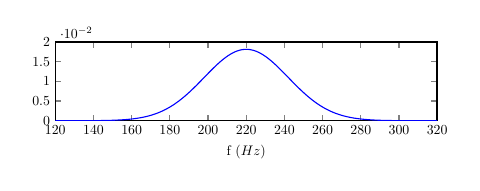
\begin{tikzpicture}[scale=0.5]
        \begin{axis}
            [
            xmin = 120, xmax = 320,
            ymin = 0, ymax = 0.02,
            xlabel = {f ($Hz$)},
            legend pos=outer north east,
            legend style={nodes={scale=1.2, transform shape}},
            ],
            \addplot[
                domain = 120:320,
                samples = 200,
                smooth,
                thick,
                blue,
            ]{(exp(-0.5*((x-220)/22)^2))/(22*sqrt(2*pi))};
            %\legend{$\frac{1}{22\sqrt{2\pi}}e^{-\frac{1}{2}(\frac{x-220}{22})^2}$};

        \end{axis}
    \end{tikzpicture}

    \caption{\textbf{Input distribution.} The input frequency representing $p(t)$ is sampled from a normal distribution with $\mu=220$ and $\sigma=22$}
    \label{fig:ModelInput}
        %\end{wrapfigure}
\end{figure}

\subsubsection{Model Output}
The simulated data from $y_1-y_2$ while varying $C$ looks like this:
\begin{figure}[H]
    \centering
    \begin{tikzpicture}
        \pgfplotsset{
        %% Axis
            scale only axis,
            width=0.8\linewidth,
            height=2cm,
            every axis/.append style={
                line width=1pt,
                tick style={line width=0.8pt},
                %   grid style={dashed, black!20},
                %  grid=major,
            },
%               %% X-Axis
            xmin=1.0,
            xmax=3,
        }
        \begin{groupplot}
            [
            group style={
                group size=1 by 6,
                vertical sep=2mm,
                xlabels at=edge bottom,
                xticklabels at=edge bottom,
            },
            yticklabel style={
                /pgf/number format/fixed,
                /pgf/number format/precision=2
            },
            legend style={nodes={scale=0.8, transform shape}, thin},
            legend image post style={scale=0},
            xlabel=$t(s)$
            ]
%           \pgfplotsinvokeforeach{0,1,2,3,4,5}{
%             \nextgroupplot
%             \addplot [line width=1pt,solid,color=cyan] table[x=x,y= c#1 ,col sep=comma]{data/test135.csv};
%          }
            \nextgroupplot
            \addplot [line width=1pt,solid] table[x=x,y=c0 ,col sep=comma]{data/simple_c_sweep.csv};
            \legend{$C=68$};
            \nextgroupplot
            \addplot [line width=1pt,solid] table[x=x,y=c1 ,col sep=comma]{data/simple_c_sweep.csv};
            \legend{$C=128$};
            \nextgroupplot
            \addplot [line width=1pt,solid] table[x=x,y=c2 ,col sep=comma]{data/simple_c_sweep.csv};
            \legend{$C=135$};
            \nextgroupplot[ylabel=v ($mV$), every axis y label/.append style={at=(ticklabel cs:1.0)}]
            \addplot [line width=1pt,solid] table[x=x,y=c3 ,col sep=comma]{data/simple_c_sweep.csv};
            \legend{$C=270$};
            \nextgroupplot
            \addplot [line width=1pt,solid] table[x=x,y=c4 ,col sep=comma]{data/simple_c_sweep.csv};
            \legend{$C=675$};
            \nextgroupplot
            \addplot [line width=1pt,solid] table[x=x,y=c5 ,col sep=comma]{data/simple_c_sweep.csv};
            \legend{$C=1350$};

        \end{groupplot}
    \end{tikzpicture}

    \caption{\textbf{Model Output for varying $C$.} Well defined alpha-activity is visible at $C=135$.}
    \label{fig:JansenRitOutput}
\end{figure}

\todo{Explain Graph, generally provide more information to the systems output}

\pagebreak

\subsection{The David and Friston Model}\label{subsec:the-david-and-friston-model}
\incomplete{the whole David-Friston-Section is still very much preliminary}

While the Jansen-Rit model succeeds in generating realistic alpha activity, real EEG Signals contain much richer spectra \parencite{steriade_impact_2001}. David and Fristion \cite{david_neural_2003} proposed a modification to the Jansen-Rit model, that could produce a more realistic frequency spectrum by introducing sub-populations to the model. They can be tuned individually to produce oscillations in different frequencies.

\subsubsection{Introducing sub-populations}

David and Friston slightly redefine $h(t)$ by introducing the parameters $H$ and $\tau$ (see Table \ref{tab:davidfriston}), which is just a minor alteration of $A$ and $a$.
\[ h(t)=Aate^{-at} => h(t)=\frac{H}{\tau}te^{-\frac{1}{\tau}} \]
Furthermore, as they are tweaking these parameters to produce slower or faster subpopulations, they define the products $H_e\tau_e=0.0325mVs$ and $H_i\tau_i=0.44mVs$ as constants. This is done to preserve the oscillatory behavior of each population \parencite{david_neural_2003}. When varying $\tau$, $H$ is therefore adjusted accordingly ($H_e=\frac{0.0325mVs}{\tau_e}$, $H_i=\frac{0.44mVs}{\tau_i}$).
\begin{table}[H]
    \centering
    \begin{tabular}{ |c|c|c|c|c| }
        \hline
        \multicolumn{2}{|c|}{Parameter} & Value & Unit & Relation to \parencite{jansen_electroencephalogram_1995} \\
        \hline
        \hline
        \rule{0pt}{3ex}Excitatory delays        & \(\tau_e\) & \(0.01\) & $s$  & $ \tau_e = \frac{1}{a} $ \\[1.2ex]
        \hline
        \rule{0pt}{3ex}Inhibitory delays        & \(\tau_i\) & \(0.02\) & $s$  & $ \tau_i = \frac{1}{b} $\\[1.2ex]
        \hline
        \rule{0pt}{3ex}Excitatory synaptic gain & \(H_e\)    & \(3.25\) & $mV$ & $ H_e = A $ \\[1.2ex]
        \hline
        \rule{0pt}{3ex}Inhibitory synaptic gain & \(H_i\)    & \(22\)   & $mV$ & $ H_i = B $ \\[1.2ex]
        \hline
    \end{tabular}
    \caption{Parameters of the PSP Blocks after \parencite{david_neural_2003}}
    \label{tab:davidfriston}
\end{table}
\fcolorbox{red}{red!10}{\parbox{\textwidth}{\textbf{Attention:} From now on, the indices $[0,...,N]$ for $y$, $h$, $\tau$ and $H$ refer only to the subpopulations within a single population. The indices used above in the formulation for the Simple Jansen-Rit Model (and the Block Diagram) should not be confused with these.
However, $e$ and $i$ as indices still denote excitatory and inhibitory populations respectively.}} \\[2em]
By introducing subpopulations, we split up the general impulse response function $h(t)$ in $N$ individual subfunctions:
\[h_n(t) = \frac{H_n}{\tau_n}te^{-\frac{1}{\tau_n}}\] \\[1em]

The previously defined general PSP-Block Equation:
\[y(t)=h(t)\ast x(t)\]
then becomes:
\[y(t)=\sum_{n=0}^{N}{(w_n \cdot h_n(t) \ast x(t))} \hspace{2em}\text{with}\hspace{2em} \sum_{n=0}^{N}w_n = 1 \hspace{2em}\text{and}\hspace{2em} 0 \leq w_n \leq 1\]
with N individually weighted ($w_n$) and parameterized ($h_n(t)$) subpopulations. \\
We can then declare:
\[y_n(t) = h_n(t) \ast x(t) \quad \text{and} \quad y(t) = \sum_{n=0}^{N} (w_ny_n)\]
which produces the following differential equations for a single PSP Block:

\begin{equation}
    \begin{aligned}
        \dot{y}_0(t) &= z_0(t) \\
        \dot{z}_0(t) &= \frac{H_0}{\tau_0} x(t) - \frac{2}{\tau_0}z_0(t) - \left(\frac{1}{\tau_0}\right)^2y_0(t)\\
        &...\\
        \dot{y}_N(t) &= z_N(t) \\
        \dot{z}_N(t) &= \frac{H_N}{\tau_N} x(t) - \frac{2}{\tau_N}z_N(t) - \left(\frac{1}{\tau_N}\right)^2y_N(t)\\
        y(t)         &= w_1y_1 + ... + w_Ny_N\\
    \end{aligned}\label{eq:davidfriston_subpops}
\end{equation}
David and Friston further propose an example with two subpopulations for each population with the following parameters: $\tau_{e_1}=10.8ms$, $\tau_{i_1}=22ms$, $\tau_{e_2}=4.6ms$, $\tau_{i_2}=2.9ms$. While the kinetics for the first subpopulation were still close to those of the original populations ($\tau_e=10ms, \tau_i=20ms$, which produce alpha-activity), the second population's parameters were chosen to produce gamma activity.

\todo{put the values in a table}

\begin{figure}[H]
    \begin{tikzpicture}
	\node(sout){};
	\node[shape=rectangle, draw=black, left=0.3cm of sout.center] (SigmPC) {$x(t)$};
	
	\node[shape=rectangle, draw=black, above right=1cm and 2.5cm of sout.center] (H1) {$h_{e_0}(t)$};
	\node[shape=rectangle, draw=black, fill=white, below right=0.2cm and 0.2cm of H1.west] (H2) {$h_{e_1}(t)$};
	\node[shape=rectangle, draw=black, fill=white, below right=2cm and 0.8cm of H2.west] (HN) {$h_{e_N}(t)$};
	\draw[black!80, linedots, linedot diameter=4pt, linedot spacing=25pt, shorten <=8pt, shorten >=8pt] (H2.south) --
    (HN.north);
	\node[shape=rectangle, dotted, draw=black, fill=white, fill opacity=0.7, text opacity=1, below right=0.8cm and 0.4cm of H2.west] (Hen) {$h_{e_n}(t)$};
	
	
	\node[left=0.3cm of H1.west](x1){};
	\node[left=0.45cm of H2.west](x2){};
	\node[left=0.85cm of Hen.west](xen){};
	\node[left=1.3cm of HN.west](xN){};
	
	\node[shape=circle, draw=black, right=2cm of H1] (w1) {\small$w_0$};
	\node[shape=circle, draw=black,fill=white, right=2cm of H2] (w2) {\small$w_1$};
	\node[shape=circle, dotted, draw=black, right=2cm of Hen] (wen) {\small$w_n$};
	\node[shape=circle, draw=black, right=2cm of HN] (wN) {\small$w_N$};
	
	
	\node[right=1.1cm of w1.east](y1){};
	\node[right=0.9cm of w2.east](y2){};
	\node[right=0.5cm of wen.east](yen){};
	\node[right=0.001cm of wN.east](yN){};
	
	\node[shape=rectangle, draw=black, right=10cm of sout.center] (pout){$y(t)$};
	
	
	\draw[-] (SigmPC.east) -- (sout.center);
	
	\draw[-] (sout.center) .. controls +(3:1.2) and +(10:-1.5) .. (x1.center);
	\draw[-] (sout.center) .. controls +(3:1.2) and +(10:-1.5) .. (x2.center);
	\draw[-, dotted] (sout.center) .. controls +(3:1.2) and +(10:-1.5) .. (xen.center);
	\draw[-] (sout.center) .. controls +(3:1.2) and +(10:-1.5) .. (xN.center);
	
	
	\draw[->] (x1.center) |- (H1.west);
	\draw[->] (x2.center) |- (H2.west);
	\draw[->, dotted] (xen.center) |- (Hen.west);
	\draw[->] (xN.center) |- (HN.west);
	
	\draw[->] (H1.east) -- (w1.west) node [above, midway]{\tiny$y_0(t)$};
	\draw[->] (H2.east) -- (w2.west)node [above, midway]{\tiny$y_1(t)$};
	\draw[->, dotted] (Hen.east) -- (wen.west)node [above, midway]{\tiny$y_n(t)$};
	\draw[->] (HN.east) -- (wN.west)node [above, midway]{\tiny$y_N(t)$};
	
	
	
	\draw[-] (w1.east) |- (y1.center);
	\draw[-] (w2.east) |- (y2.center);
	\draw[-, dotted] (wen.east) |- (yen.center);
	\draw[-] (wN.east) |- (yN.center);
	
	\draw[->, very thin] (y1.center) .. controls +(3:1.2) and +(10:-1.5) .. (pout.west);
	\draw[->, very thin] (y2.center) .. controls +(3:1.2) and +(10:-1.5) .. (pout.west);
	\draw[->, dotted, thin] (yen.center) .. controls +(3:1.2) and +(10:-1.5) .. (pout.west);
	\draw[->, very thin] (yN.center) .. controls +(3:1.2) and +(10:-1.5) .. (pout.west);
	
\end{tikzpicture}
    \caption{Example of subpopulations ($h_{e_0}(t), ..., h_{e_N}(t)$) forming an excitatory population $h_e(t)$}
    \label{fig:exc_subpops}
\end{figure}
%\subsection{möglicherweise auch vorangegangene Paper (Lopez da Silva '76, ...) zur Erklärung heranziehen}
%
%\subsection{ Was sind die Erweiterungen von (David and Friston 2003)?}
%\subsection{An welcher Stelle können wir in dem Modell Sedation modellieren?}

\subsection{New PSP Functions}\label{subsec:new-psp-functions}

\begin{figure}[H]
    \centering
    \pgfplotsset{compat = newest}
    \begin{tikzpicture}
        \begin{axis}
            [
            xmin = -1, xmax = 140,
            ymin = 0, ymax = 15.1,
            xlabel = {$t$ ($ms$)},
            ylabel = {$h$ ($mV$)},
            legend pos=north east,
            legend style={nodes={scale=0.8, transform shape}},
            domain = 0:140,
            samples = 200,
            smooth,
            thick,
            ],
            \addplot[green] {(3.01/10.8)*x*e^(-(1/10.8)*x)};\label{plot:line1}
            \addplot[lime] {(7.07/4.6)*x*e^(-(1/4.6)*x)};\label{plot:line2}
            \addplot[red] {(20/22)*x*e^(-(1/22)*x)};\label{plot:line3}
            \addplot[magenta] {(151.72/2.9)*x*e^(-(1/2.9)*x)};\label{plot:line4}
%
%            \addplot[red, dashed] {(20/22)*x*e^(-(1/22)*x)};\label{plot:line5}
%            \addplot[red, dashed] {(20/24.2)*x*e^(-(1/24.2)*x)};\label{plot:line5.1}
%            \addplot[red, dashed] {(20/26.4)*x*e^(-(1/26.4)*x)};\label{plot:line5.2}
%            \addplot[red, dashed] {(20/28.6)*x*e^(-(1/28.6)*x)};\label{plot:line5.3}
%            \addplot[red, dashed] {(20/30.8)*x*e^(-(1/30.8)*x)};\label{plot:line5.4}
%            \addplot[red, dashed] {(20/33)*x*e^(-(1/33)*x)};\label{plot:line5.5}
%
%            \addplot[magenta, dashed] {(151.72/2.9)*x*e^(-(1/2.9)*x)};\label{plot:line6.1}
%            \addplot[magenta, dashed] {(151.72/3.19)*x*e^(-(1/3.19)*x)};\label{plot:line6.2}
%            \addplot[magenta, dashed] {(151.72/3.48)*x*e^(-(1/3.48)*x)};\label{plot:line6.3}
%            \addplot[magenta, dashed] {(151.72/3.77)*x*e^(-(1/3.77)*x)};\label{plot:line6.4}
%            \addplot[magenta, dashed] {(151.72/4.06)*x*e^(-(1/4.06)*x)};\label{plot:line6.5}
%            \addplot[magenta, dashed] {(151.72/4.35)*x*e^(-(1/4.35)*x)};\label{plot:line6.6}
            \coordinate (legend) at (axis description cs:0.97,0.97);
        \end{axis}
        \tiny
        \matrix [
            draw,
            matrix of nodes,
            anchor=north east,
        ] at (legend) {

            & $\tau$ &    $H$  \\
            $h_{e_1}(t)$~\ref{plot:line1} & 10.8ms &   3.0mV \\
            $h_{e_2}(t)$~\ref{plot:line2} &  4.6ms &   7.0mV \\
            $h_{i_1}(t)$~\ref{plot:line3} & 22.0ms &  20.0mV \\
            $h_{i_2}(t)$~\ref{plot:line4} &  2.9ms & 151.7mV \\
        };
    \end{tikzpicture}

    \caption{\textbf{PSP functions for Subpopulations:}~\ref{plot:line2} and~\ref{plot:line4} are faster
    subpopulations} \
    \label{fig:PSPPlotDavidFriston}
\end{figure}    
